\documentclass[a4paper]{article}
\usepackage{a4wide,amssymb,epsfig,latexsym,multicol,array,hhline,fancyhdr}
\usepackage{vntex}
\usepackage{amsmath}
\usepackage{lastpage}
\usepackage[lined,boxed,commentsnumbered]{algorithm2e}
\usepackage{enumerate}
\usepackage{color}
\usepackage{graphicx}							% Standard graphics package
\usepackage{array}
\usepackage{tabularx, caption}
\usepackage{multirow}
\usepackage{multicol}
\usepackage{rotating}
\usepackage{graphics}
\usepackage{geometry}
\usepackage{setspace}
\usepackage{caption}
\usepackage{subcaption}
\usepackage{epsfig}
\usepackage{tikz}
\usetikzlibrary{arrows,snakes,backgrounds}
\usepackage{hyperref}
\hypersetup{urlcolor=blue,linkcolor=black,citecolor=black,colorlinks=true} 
%\usepackage{pstcol} 								% PSTricks with the standard color package

\newtheorem{theorem}{{\bf Theorem}}
\newtheorem{property}{{\bf Property}}
\newtheorem{proposition}{{\bf Proposition}}
\newtheorem{corollary}[proposition]{{\bf Corollary}}
\newtheorem{lemma}[proposition]{{\bf Lemma}}

\AtBeginDocument{\renewcommand*\contentsname{Mục lục}}
\AtBeginDocument{\renewcommand*\refname{References}}
%\usepackage{fancyhdr}
\setlength{\headheight}{40pt}
\pagestyle{fancy}
\fancyhead{} % clear all header fields
\fancyhead[L]{
	\begin{tabular}{rl}
		\begin{picture}(25,15)(0,0)
			\put(0,-8){
\includegraphics[width=8mm, height=8mm]{images/hcmut.png}}
			%\put(0,-8){\epsfig{width=10mm,figure=hcmut.eps}}
		\end{picture}&
		%
\includegraphics[width=8mm, height=8mm]{hcmut.png} & %
		\begin{tabular}{l}
			\textbf{\bf \ttfamily Đại học Bách Khoa TP.HCM}\\
			\textbf{\bf \ttfamily Khoa Khoa học và Kĩ thuật Máy tính}
		\end{tabular} 	
	\end{tabular}
}
\fancyhead[R]{
	\begin{tabular}{l}
		\tiny \bf \\
		\tiny \bf 
\end{tabular}  }
\fancyfoot{} % clear all footer fields
\fancyfoot[L]{\scriptsize \ttfamily Bài tập lớn môn Mạng Máy Tính (CO3093) - Năm học 2023 - 2024}
\fancyfoot[R]{\scriptsize \ttfamily Trang {\thepage}/\pageref{LastPage}}
\renewcommand{\headrulewidth}{0.3pt}
\renewcommand{\footrulewidth}{0.3pt}


%%%
\setcounter{secnumdepth}{4}
\setcounter{tocdepth}{3}
\makeatletter
\newcounter {subsubsubsection}[subsubsection]
\renewcommand\thesubsubsubsection{\thesubsubsection .\@alph\c@subsubsubsection}
\newcommand\subsubsubsection{\@startsection{subsubsubsection}{4}{\z@}%
	{-3.25ex\@plus -1ex \@minus -.2ex}%
	{1.5ex \@plus .2ex}%
	{\normalfont\normalsize\bfseries}}
\newcommand*\l@subsubsubsection{\@dottedtocline{3}{10.0em}{4.1em}}
\newcommand*{\subsubsubsectionmark}[1]{}
\makeatother


\begin{document}
	
	\begin{titlepage}
		\begin{center}
			ĐẠI HỌC QUỐC GIA TP.HCM \\
			ĐẠI HỌC BÁCH KHOA TP.HCM \\
			KHOA KHOA HỌC VÀ KĨ THUẬT MÁY TÍNH
		\end{center}
		
		\vspace{1cm}
		
		\begin{figure}[h!]
			\begin{center}
				
\includegraphics[width=3cm]{images/hcmut.png}
			\end{center}
		\end{figure}
		
		\vspace{1cm}
		
		
		\begin{center}
			\begin{tabular}{c}
				\multicolumn{1}{l}{\textbf{{\Large MẠNG MÁY TÍNH (CO3093)}}}\\
				~~\\
				\hline
				\\
				\multicolumn{1}{l}{\textbf{{\Large Assignment 1}}}\\
				\\
				\textbf{{\Huge Develop a Network Application}}\\
				\\
				\hline
			\end{tabular}
		\end{center}
		
		\vspace{3cm}
		
		\begin{table}[h]
			\begin{tabular}{rrl}
				\hspace{5 cm} & Giảng viên hỗ trợ: & Nguyễn Phương Duy\\
				& Sinh viên: & Nguyễn Thành Đạt - 2111018 \\
				& & Tạ Nguyễn Tiến Dũng - 2110965 \\
				& & Nguyễn Duy Hà - 2011130 \\
				& & Nguyễn Việt Anh - 2112801
			\end{tabular}
		\end{table}
		
		\begin{center}
			{\footnotesize Thành phố Hồ Chí Minh, Tháng 12 năm 2020}
		\end{center}
	\end{titlepage}
	
	
	%\thispagestyle{empty}
	
	\newpage
	\tableofcontents
	\newpage
	
	
	%%%%%%%%%%%%%%%%%%%%%%%%%%%%%%%%%
	\section{Member list \& Workload}
	
	\begin{center}
		\begin{tabular}{|c|c|c|l|c|}
			\hline
			\textbf{No.} & \textbf{Fullname} & \textbf{Student ID} & \textbf{Problems} & \textbf{Percentage of work}\\
			\hline 
			%%%%%Student 1%%%%%%%%%%
			\multirow{3}{*}{1} & \multirow{3}{*}{Nguyễn Thành Đạt} & \multirow{3}{*}{2111018} & - Code chính & \multirow{3}{*}{30\%}\\
			& &  & - Testing &\\
			& &  & &\\
			\hline 
			%%%%%Student 2%%%%%%%%%%%
			\multirow{3}{*}{2} & \multirow{3}{*}{Tạ Nguyễn Tiến Dũng} & \multirow{3}{*}{2110965} & - Vẽ sơ đồ, thiết kế hệ thống & \multirow{3}{*}{25\%}\\
			& &  & &\\
			& &  & &\\
			\hline
			%%%%%Student 3%%%%%%%%%%%
			\multirow{3}{*}{2} & \multirow{3}{*}{Nguyễn Duy Hà} & \multirow{3}{*}{2011130} & - Hỗ trợ code & \multirow{3}{*}{20\%}\\
			& &  & - Mô tả yêu cầu chương trình &\\
			& &  & &\\
			\hline
			%%%%%Student 4%%%%%%%%%%%
			\multirow{3}{*}{2} & \multirow{3}{*}{Nguyễn Việt Anh} & \multirow{3}{*}{2112801} & - Viết báo cáo & \multirow{3}{*}{25\%}\\
			& &  & &\\
			& &  & &\\
			\hline
		\end{tabular}
	\end{center}
	
	%%%%%%%%%%%%%%%%%%%%%%%%%%%%%%%%%
	\section{Application specifications and requirements}
	\subsection{Project objectives}
	$\indent$Mục đích của bài tập lớn môn Mạng Máy tính học kì 1 năm học 2023-2024 là xây dựng một chương trình chia sẻ file đơn giản, với giao thức chương trình do mỗi nhóm quyết định, dựa trên các giao thức TCP/IP đã học.
	
	\subsection{Project specifications and description}
	$\indent$ Mô tả chương trình trong đề bài bài tập lớn 1:
	\begin{itemize}
		\item Một máy chủ (server) trung tâm đóng vai trò theo dõi, quản lí các client đã kết nối và các file mà chúng giữ.
		\item Một client sẽ thông báo cho server biết có những file gì trong thư mục tại chổ (local repository) nhưng sẽ không truyền những file đó cho server.
		\item Khi một client cần một file không nằm trong thư mục của nó, môt yêu cầu sẽ được gửi đến server. Server có nhiệm vụ xác định những clients khác có chứa file được yêu cầu và gửi thông tin kết nối của chúng đến client yêu cầu. Client đó sẽ lựa chọn nguồn lấy phù hợp và tiến hành nhận file trực tiếp từ đó mà không qua can thiệp của server. (Loại mạng kết nối Peer-to-peer)
		\item Nhiều client có thể tải nhiều file khác nhau từ cùng một client gốc tại bất kì thời điểm nào
		\item Client có giao diện câu lệnh (Command line interface - CLI) đơn giản nhận hai câu lệnh:
		\begin{itemize}
			\item \textbf{publish \textit{lname fname}}: một file trong file system của client đã được thêm vào local repository của client đó và thông tin này được truyền đến cho server.
			\item \textbf{fetch \textit{fname}}: lấy một bản copy từ file mục tiêu và thêm nó vào local repository.
		\end{itemize}
		\item Server cũng sẽ có CLI nhận hai câu lệnh:
		\begin{itemize}
			\item \textbf{discover \textit{hostname}}: cho ra danh sách những file trong local repository của \textit{hostname}.
			\item \textbf{ping \textit{hostname}}: kiểm tra trực tiếp \textit{hostname}, tương tự như câu lệnh SNMP ping.
		\end{itemize}
	\end{itemize}
	$\indent$Bên cạnh đó, dựa trên ý kiến của các thành viên, nhóm có thêm các yêu cầu dựa trên các chức năng thêm và cách xử lí khi gặp các trường hợp đăc biệt:
	\begin{itemize}
		\item Với các câu lệnh bên phía client:
		\begin{itemize}
			\item Câu lệnh \textbf{publish \textit{lname fname}} sẽ tiến hành thêm file từ trong máy của client vào local repo và thông báo tới server .Nếu publish một file không tồn tại sẽ báo lỗi "File not exist!". Nếu file publish đã nằm trong local repo sẵn rồi báo "File already in local repo!".
			\item Cách xử lí của câu lệnh \textbf{fetch \textit{fname}} của client trong các trường hợp
			\begin{enumerate}
				\item Nếu file đó không nằm trong hệ thống server quản lí thì báo lỗi "File not recognized!"
				\item Nếu file đó đã nằm trong repo của client thì thông báo đã file đã tồn tại trong local repository
				\item Nếu file đó không nằm trong repo thì thực hiện theo như đề bài yêu cầu
				\item Nếu client chứa file đó không kết nối được thì báo lỗi kết nối 
			\end{enumerate}
			Bên cạnh đó, việc fetch một file vào local repository cũng sẽ đồng thời thông báo với server, tức là file tên \textit{fname} có mặt trên ít nhất hai client.
			\item Thêm câu lệnh \textbf{delete \textit{filename}}: Xóa một file từ local repo ra khỏi hệ thống i.e server sẽ không còn lưu thông tin về file này trên client nữa.
			Báo lỗi "Cannot delete! File not in local repo!" nếu file đó không nằm trong local repo của client yêu cầu. Tức là một client chỉ có thể xóa một file trong local repo của bản thân.
			\item Thêm câu lệnh \textbf{discover \textit{hostname}}: In ra danh sách file mà \textit{hostname} đã publish trên server. Nếu một \textit{hostname} chưa từng kết nối với server từ trước thì báo lỗi "Host not recognize!". Nếu \textit{hostname} đã kết nối nhưng chưa publish bất kì file thì báo "\textit{hostname} has not published any files!".
			\item Thêm câu lệnh \textbf{list}: In ra danh sách các client đã từng kết nối với server. Khi đó một client kết hợp câu lệnh này với câu lệnh \textbf{discover \textit{hostname}} để tìm được file mình muốn chuyển.
		\end{itemize}
		\item Với câu lệnh bên phía server:
		\begin{itemize}
			\item Lưu ý của câu lệnh \textbf{discover \textit{hostname}}:Chức năng và lưu ý tương tự như với câu lệnh ở bên client. 
			\item \textbf{ping \textit{hostname}}: Tương tự như câu lệnh ping trong command prompt, gửi vài packet/message nhỏ đến \textit{hostname} rồi chờ phản hồi.
		\end{itemize}
		\item Client sẽ biết trước thông tin kết nối của server.
		\item Client cần có cơ chế tạo, quản lí nhiều cổng kết nối sử dụng đa luồng để nhiều client có thể lấy file từ một client cùng lúc.
		\item Các client không cần liên tục kết nối với server để thực hiện việc truyền file, miễn là vẫn nằm trong cùng một network.
		\item Server lưu thông tin về các client đã kết nối cũng như các file họ đã publish trong hệ dữ liệu của chính nó (tức là nếu tắt server đi thì dữ liệu này cũng sẽ biến mất).
		\item Server cũng cần có cơ chế tạo, quản lí nhiều cổng kết nối cùng một lúc.
		\item Có thể có nhiều bản copy của một file trên nhiều client khác nhau. Tức là một tên file có thể tồn tại ở nhiều client khác nhau
		\item Hệ thống không nhận diện các file trùng lặp trong local repo của client. Tức là kể cả khi client có nhiều file trùng lặp thì hệ thống ghi nhận chỉ một file trong local repo. (\textbf{publish \textit{lname fname}} không cho phép file trùng lặp được publish lên server)
	\end{itemize}
	
	%%%%%%%%%%%%%%%%%%%%%%%%%%%%%%%%%
	\section{System modeling and architecture design}
	\subsection{General use-case diagram}
	$\indent$Hệ thống có 2 actor, bao gồm server và client. Bên cạnh đó, hệ thống cũng có hai module xử lí hai dịch vụ khác nhau của chương trình: quản lí file và client (clients and files management), truyền file (file transfer). Với mỗi module đó là các use-case ứng với mỗi câu lệnh và chức năng của từng actor.
	\begin{figure}[h]
		\begin{center}
			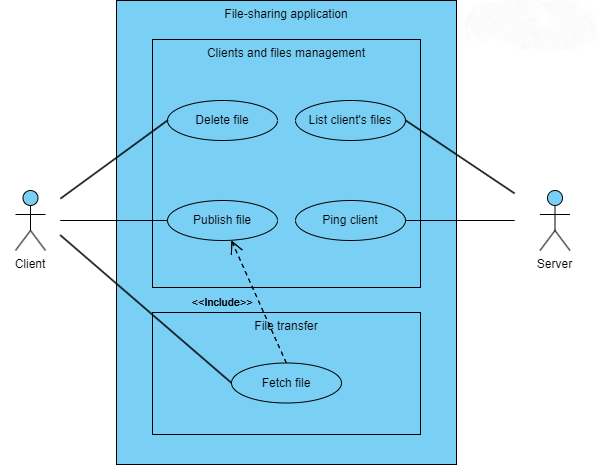
\includegraphics[width=\textwidth]{images/Gen_usecase_diagram.png}
			\hspace{\textwidth}
			\caption{Lược đồ use-case tổng quát}
			\label{usecase_diagram}
		\end{center}
	\end{figure}
	\subsection{Activity diagram main functions}
	$\indent$Ứng với mỗi câu lệnh (use-case) chính của từng actor, ta có được các lược đồ hoạt động (activity diagram) dưới đây. Ở đây lưu ý, khi lược đồ đi đến final node thì cũng đồng thời đóng mọi kết nối socket đã thiết lập trước đó, nhằm tránh việc tạo quá nhiều kết nối không cần thiết.
	\subsubsection{publish \textit{lname fname}}
	$\indent$Client sẽ đầu tiên gửi yêu cầu kết nối với server, server sẽ lắng nghe yêu cầu từ một socket đang chạy của mình, thiết lập kết nối giữa client và server. Sau đó, client thực hiện việc publish file lên dữ liệu của server. Kiểm tra tại client file đó có tồn tại không. Nếu có thì tiếp tục use-case, không thì báo lỗi và kết thúc. Sau đó, server sẽ kiểm tra xem client này đã publish file này vào local repo trước đó chưa. Nếu có rồi thì báo lỗi và kết thúc, nếu không thì tiếp tục use-case. Server sẽ thêm file đó vào dữ liệu của mình và client thì thêm file đó vào local repo trên máy. Cuối cùng là đóng kết nối và kết thúc use-case.
	\begin{figure}[!h]
		\begin{center}
			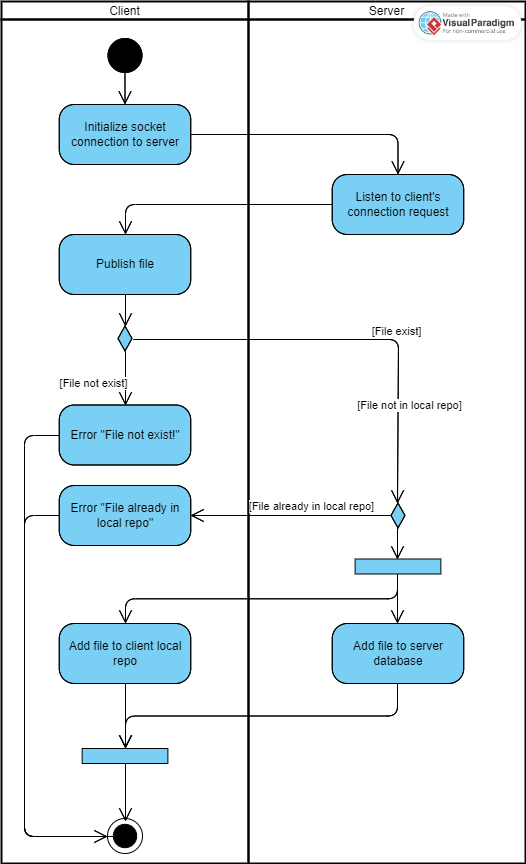
\includegraphics[width=0.5\textwidth]{images/publish_activity_diagram.png}
			\hspace{\textwidth}
			\caption{Lược đồ hoạt động của câu lệnh \textbf{publish \textit{lname fname}}}
			\label{publish_diagram}
		\end{center}
	\end{figure}
	\subsubsection{fetch \textit{fname}}
	$\indent$Thiết lập kết nối tương tự như \textbf{publish}. Tuy nhiên, trong lúc implement thực tế chương trình, nhóm có sửa đổi thứ tự hoạt động khác lược đồ một chút để thuận tiện cho việc code. Trong đó, sau khi client gửi yêu cầu fetch file, server sẽ kiểm tra file đó đã có trong local repo chưa. Nếu có rồi thì báo lỗi và kết thúc, nếu không thì tiếp tục use-case. Sau đó, server tiến hành tìm client có file được yêu cầu. Nếu không tìm được i.e file không nằm trong dữ liệu server thì báo lỗi và kết thúc, còn nếu tìm được thì gửi thông tin kết nối của target client cho client yêu cầu. Sau đó client yêu cầu thiết lập kết nối với target client và tiến hành truyền file. Cuối cùng, đóng mọi socket đã thiêt lập (cả với server và target client).
	\begin{figure}[!h]
		\begin{center}
			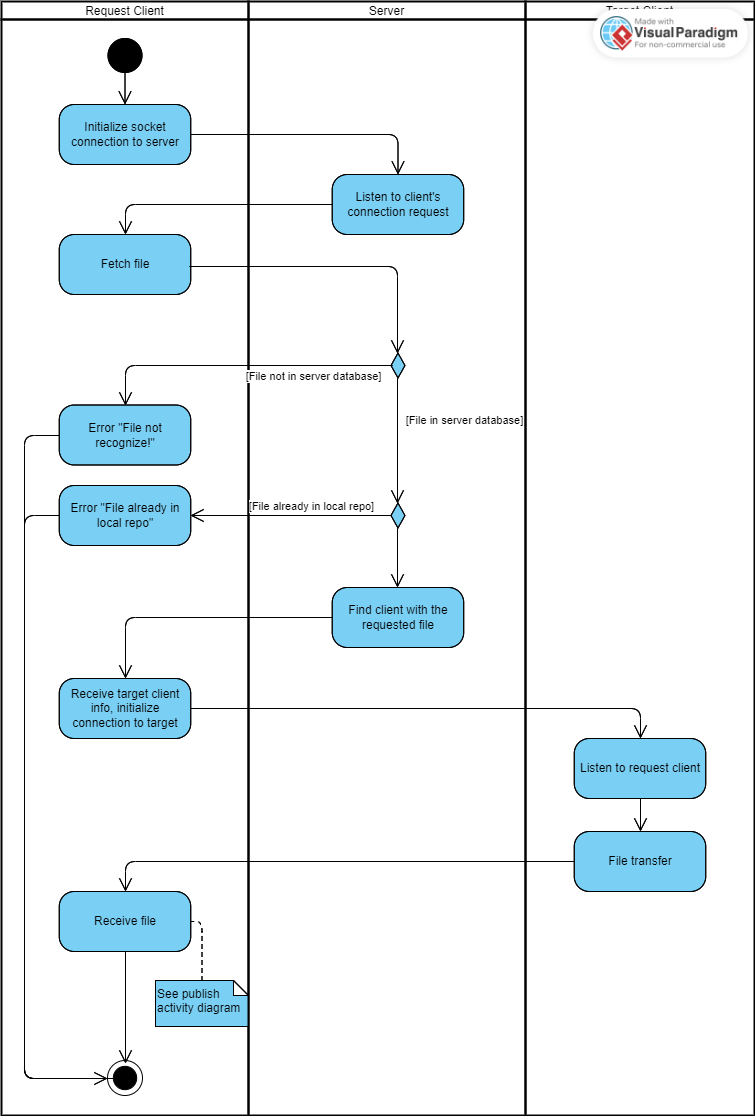
\includegraphics[width=0.6\textwidth]{images/fetch_activity_diagram.png}
			\hspace{\textwidth}
			\caption{Lược đồ hoạt động của câu lệnh \textbf{fetch \textit{fname}}}
			\label{fetch_diagram}
		\end{center}
	\end{figure}
	\newpage
	\subsubsection{delete \textit{fname}}
	$\indent$Thiếp lập kết nối tương tự hai câu lệnh trước. Server sẽ tiến hành kiểm tra xem file đó có trong local repo của client hay không. Trường hợp có thì tiến hành xóa khỏi dữ liệu server, trường hợp không thì đóng kết nối và kết thúc.
	\begin{figure}[h]
		\begin{center}
			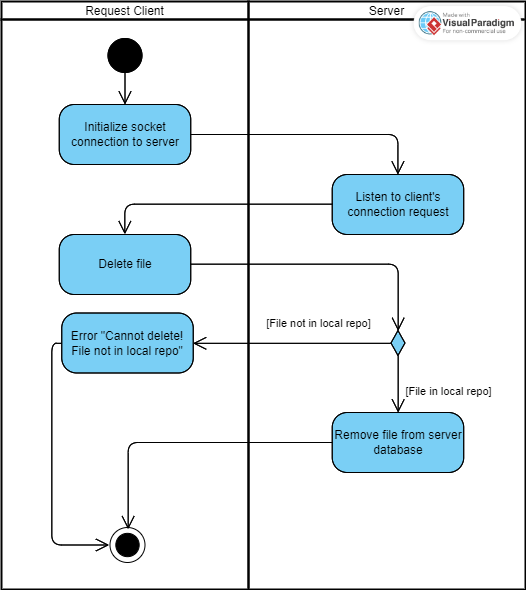
\includegraphics[width=0.7\textwidth]{images/delete_activity_diagram.png}
			\hspace{\textwidth}
			\caption{Lược đồ hoạt động của câu lệnh \textbf{delete \textit{fname}}}
			\label{delete_diagram}
		\end{center}
	\end{figure}
	\subsubsection{discover \textit{hostname} (Client side)}
	$\indent$Client gửi dữ liệu tới server về \textit{hostname}. Server sẽ kiểm tra xem nếu \textit{hostname} đã từng kết nối từ trước chưa. Nếu chưa thì thông báo lỗi và kết thúc, còn không thì gửi về client danh sách các file mà \textit{hostname} đã publish. Cách hoạt động và lưu ý khi xử lí lỗi tương tự với câu lệnh \textbf{discover \textit{hostname}} bên server.
	\newpage
	\begin{figure}[h]
		\begin{center}
			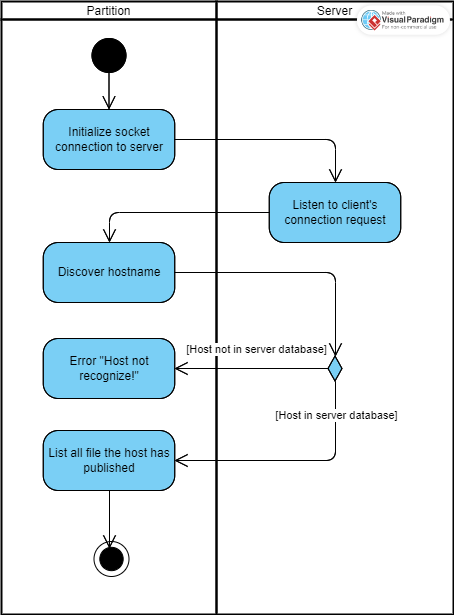
\includegraphics[width=0.7\textwidth]{images/client_discover_activity_diagram.png}
			\hspace{\textwidth}
			\caption{Lược đồ hoạt động của câu lệnh \textbf{discover \textit{hostname}} của client}
			\label{client_discover_diagram}
		\end{center}
	\end{figure}
	\subsubsection{list}
	$\indent$Client gửi yêu cầu tới server để biết về toàn bộ các client đã từng kết nối với server trước đây.
	\newpage
	\begin{figure}[!h]
		\begin{center}
			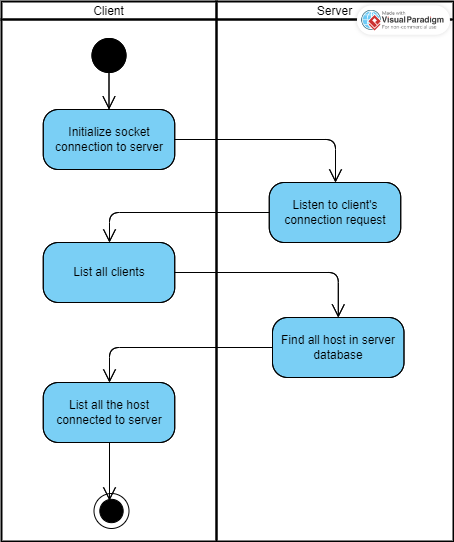
\includegraphics[width=0.7\textwidth]{images/list_activity_diagram.png}
			\hspace{\textwidth}
			\caption{Lược đồ hoạt động của câu lệnh \textbf{list}}
			\label{list_diagram}
		\end{center}
	\end{figure}
	\subsubsection{discover \textit{hostname} (Server side)}
	$\indent$Từ dữ liệu server đã nhận được từ việc các client publish file của mình lên. Server kiểm tra xem \textit{hostname} đã từng kết nối chưa. Trường hợp có rồi và đã publish file thì cho ra danh sách các file trong local repo, còn nếu chưa publish file thì cũng thông báo ra màn hình. Trường hợp chưa từng kết nối thì báo lỗi và kết thúc. Câu lệnh này chỉ cần duy nhất server thực hiện, không cần kết nối với client nào.
	\newpage
	\begin{figure}[h]
		\begin{center}
			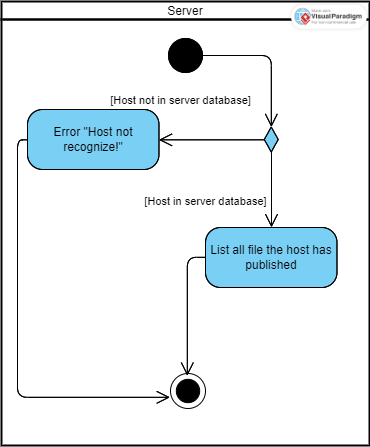
\includegraphics[width=0.7\textwidth]{images/discover_activity_diagram.png}
			\hspace{\textwidth}
			\caption{Lược đồ hoạt động của câu lệnh \textbf{discover \textit{hostname}} của server}
			\label{discover_diagram}
		\end{center}
	\end{figure}
	\subsubsection{ping \textit{hostname}}
	$\indent$Dùng để ping tới một \textit{hostname} đã kết nối với server từ trước. Nếu đã kết nối từ trước thì thực hiện việc trao đổi message xác nhận cho nhau. Còn nếu chưa thì báo lỗi và kết thúc.
	\begin{figure}[h]
		\begin{center}
			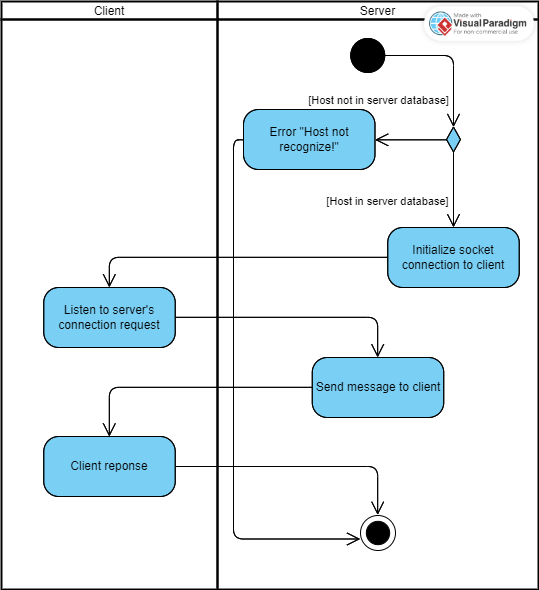
\includegraphics[width=0.7\textwidth]{images/ping_activity_diagram.png}
			\hspace{\textwidth}
			\caption{Lược đồ hoạt động của câu lệnh \textbf{ping \textit{hostname}}}
			\label{ping_diagram}
		\end{center}
	\end{figure}
	\newpage
	%%%%%%%%%%%%%%%%%%%%%%%%%%%%%%%%%
	
	
	\section{Implement and validation}
	\subsection{Manual document}\label{Manual}
	$\indent$Đây là phần hướng dẫn sử dụng ứng dụng chia sẻ file của Bài tập lớn 1 môn Mạng Máy Tính
	\subsubsection{System requirement}
	$\indent$Yêu cầu về hệ thống để ứng dụng hoạt động:
	 \begin{itemize}
	 	\item Hệ điều hành Windows có hỗ trợ Python (đã test trên Win 11, có test trên máy ảo Ubuntu 22.04). File \texttt{Client\_for\_Linux} chỉ dùng để test trên máy ảo sử dụng Linux. Trong phạm vi bài tập lớn này, ứng dụng sẽ chạy hoàn toàn trên các máy sử dụng hệ điều hành Windows.
	 	\item Cả server và client có chung mạng cục bộ (LAN - Local Area Network) với nhau, đảm bảo ping nhau qua lại được trên terminal của máy.
	 	\item Có cài đặt Python, tốt nhất là Python 3 từ bản 3.11 trở xuống (Bản 3.12 khi test đã không thể tạo được thread mới, đây là lỗi thuộc về Python Interpreter 3.12 nên nó nằm ngoài phạm vi xử lí của bài tập lớn). Đồng thời có cài đặt module "Typer" cho ứng dụng CLI.
	 \end{itemize}
	\subsubsection{Client User Configuration Requirement}
	$\indent$Yêu cầu cấu hình từ người dùng client để ứng dụng hoạt động được bình thường:
	\begin{enumerate}
		\item Trong phạm vi của bài tập lớn này, server là một máy tính cá nhân của thành viên trong nhóm, do đó địa chỉ IP của server có thể thay đổi, cần phải sửa biến global \textit{SERVER\_HOST} trên từng client.
		\item Qua module socket, Python có thể lấy được địa chỉ IP của máy client. Tuy nhiên, vì thực tế cấu hình mỗi máy có nhiều địa chỉ IP, mà địa chỉ IP thực sự dùng để kết nối lại tùy thuộc vào loại kết nối mà máy đang sử dụng (Wifi, Ethernet, ...). Do đó cần người dùng thay đổi cách lấy địa chỉ IP trong file \textit{Client.py} để chương trình có thể hoạt động:
		\begin{itemize}
			\item Tìm các địa chỉ IP của máy bằng việc gõ câu lệnh \texttt{ipconfig} vào terminal. Trên terminal sẽ có thể hiện nhiều địa chỉ IP, trong đó địa chỉ IP có trường \textbf{Default Gateway} không bị bỏ trống chính là địa chỉ IP thực sự dùng để kết nối mạng.
			\item Địa chỉ IP của máy được tìm thông qua đoạn code ở phần đầu file \texttt{Client.py}: \emph{\texttt{CLIENT\_HOST = socket.gethostbyname\_ex(socket.gethostname())[2][\textbf{X}]}}. Trong đó, \textbf{X} là thứ tự của địa chỉ IP có trường \textbf{Default Gateway} tìm thấy ở trên trong số các địa chỉ IP được terminal hiện ra.\\
			Một máy Windows có thể có nhiều địa chỉ IP bao gồm cho kết nối Ethernet, Wireless (như Wifi), WSL (Windows Subsystem for Linux),...
		\end{itemize}
	\end{enumerate}
	\subsubsection{User Guide}
	$\indent$\textbf{Dành cho Server user:}
	\begin{enumerate}
		\item Bật server bằng việc cho chạy file \textit{"Server.py"}
		\item Từ đây có thể bắt đầu sử dụng CLI của server. Chuyển terminal đến vị trí folder chứa file \textit{"Server\_app.py"}. Gọi câu lệnh (command) theo cú pháp: \texttt{py Server\_app.py} + câu lệnh
		\item CLI của server có những câu lệnh sau:
		\begin{itemize}
			\item \textbf{discover \textit{hostname}}: In ra danh sách file mà \textit{hostname} có trong local repo. Lưu ý, \textit{hostname} ở đây là địa chỉ IP.
			\item \textbf{ping \textit{hostname}}: Ping đến \textit{hostname} bằng việc gửi các gói tin và chờ phản hồi, tương tự câu lệnh ping trong terminal
		\end{itemize}
	\end{enumerate}
	$\indent$\textbf{Dành cho Client user:}
	\begin{enumerate}
		\item Bật client bằng việc cho chạy file \textit{"Client.py"}
		\item Từ đây có thể bắt đầu sử dụng CLI của client. Chuyển terminal đến vị trí folder chứa file \textit{"Client\_app.py"}. Gọi câu lệnh (command) theo cú pháp: \texttt{py Client\_app.py} + câu lệnh
		\item CLI của client có những câu lệnh sau:
		\begin{itemize}
			\item \textbf{publish \textit{lname fname}}: Thêm file tên \textit{fname} từ trong máy của client tại địa chỉ \textit{lname} vào local repo và thông báo tới server.
			\item \textbf{fetch \textit{fname}}: Lấy file tên \textit{fname} từ một trong các client đã kết nối tới server
			\item \textbf{delete \textit{filename}}: Xóa file tên \textit{fname} từ local repo ra khỏi local repo của client trong server
			\item \textbf{discover \textit{hostname}}: In ra danh sách file mà \textit{hostname} đã publish trên server.
			\item \textbf{list}: In ra danh sách các client đã từng kết nối với server. Một client có thể kết hợp câu lệnh này với câu lệnh \textbf{discover \textit{hostname}} để tìm được file mình muốn chuyển.
		\end{itemize}
		\item \textbf{Lưu ý khi sử dụng CLI:} với các trường hợp tên file hoặc tên đường dẫn có chứa khoảng trống, khi nhập vào terminal phải đóng trong dấu ngoặc kép. Khi nhập tên file cần nhập luôn cả file extension (.txt, .doc, .png, ...). Đường dẫn file sẽ là đường dẫn tuyệt đối, chỉ tới thư mục chứa file đó.
	\end{enumerate}
	\subsection{Source code}
	$\indent$Protocol trao đổi Message qua lại giữa các client và server trong việc thực hiện các câu lệnh tuân theo cú pháp: (địa chỉ IP)*(Tên câu lệnh)*(Danh sách input của câu lệnh).\\
	Về source code của chương trình, xem các file \texttt{Client.py, Client\_for\_Linux.py, Client\_app.py, Server.py, Server\_app.py} trong hai thư mục \textit{Client, Server}
	\subsection{Validation and evaluation}
	$\indent$Tiến hành việc chạy thử và kiểm tra chương trình. Thực hiện theo các bước như trong phần \ref{Manual}, tiến hành chạy các câu lệnh
	\subsubsection{Thêm và xóa file từ file system của client vào dữ liệu của server}
	Tiến hành publish ba file từ client lên server.
	\begin{figure}[h]
		\begin{center}
			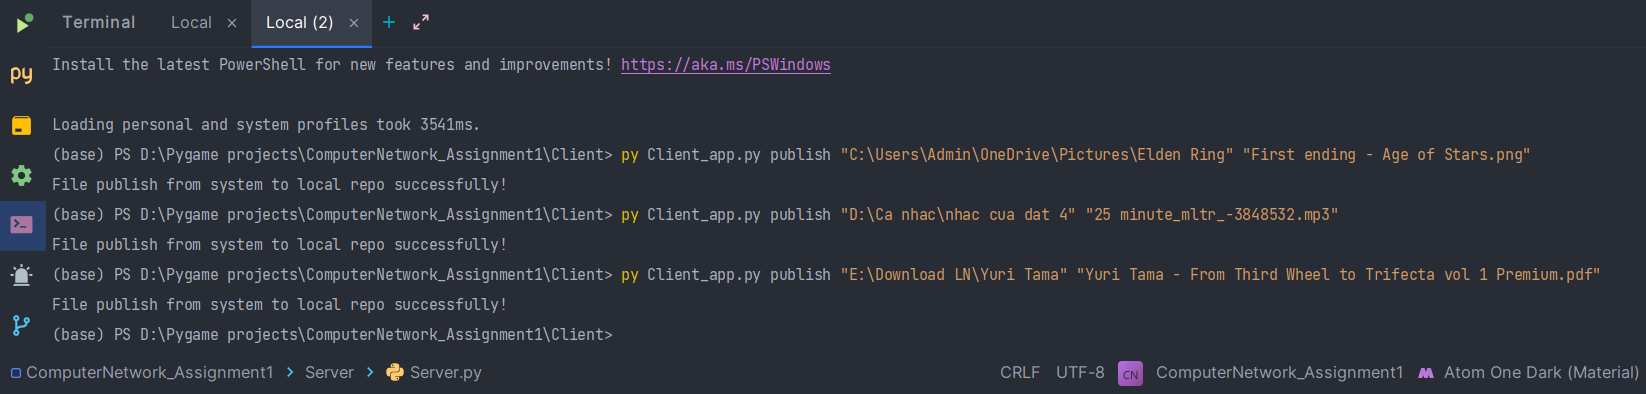
\includegraphics[width=0.8\textwidth]{tests/publish_command.png}
			\hspace{\textwidth}
			\caption{Câu lệnh \textbf{publish} từ client}
			\label{publish_command}
		\end{center}
	\end{figure}
	\begin{figure}[h]
		\begin{center}
			\begin{subfigure}[b]{0.35\textwidth}
				\centering
				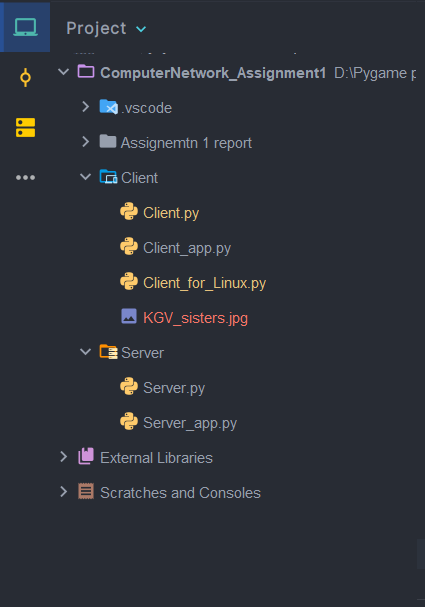
\includegraphics[width=\textwidth]{tests/client_bf_publish.png}
				\hspace{\textwidth}
				\caption{Trước khi publish}
			\end{subfigure}
			\begin{subfigure}[b]{0.35\textwidth}
				\centering
				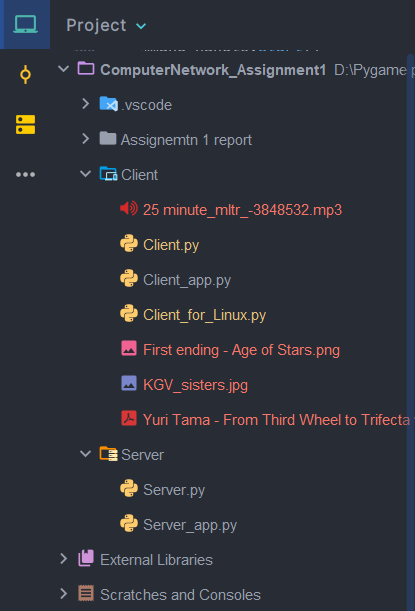
\includegraphics[width=\textwidth]{tests/client_af_publish.png}
				\hspace{\textwidth}
				\caption{Sau khi publish}
			\end{subfigure}
			\caption{Client trước và sau khi publish}
		\end{center}
	\end{figure}
	\newpage
	Kiểm tra file trên server.
	\begin{figure}[h]
		\begin{center}
			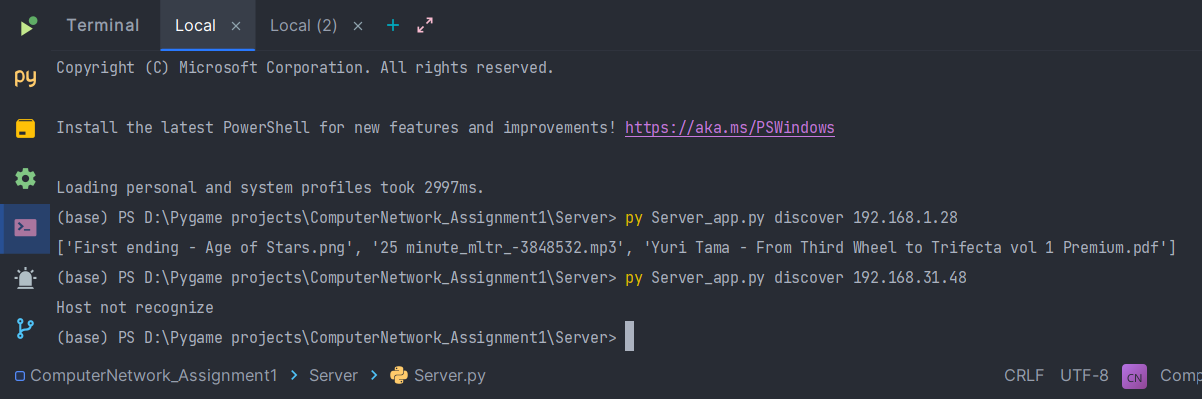
\includegraphics[width=0.7\textwidth]{tests/server_dis_af_publish.png}
			\hspace{\textwidth}
			\caption{Câu lệnh \textbf{discover} từ server}
			\label{server_dis1_command}
		\end{center}
	\end{figure}
	\\
	Sau đó, delete một file ra khỏi dữ liệu của server.
	\begin{figure}[h]
		\begin{center}
			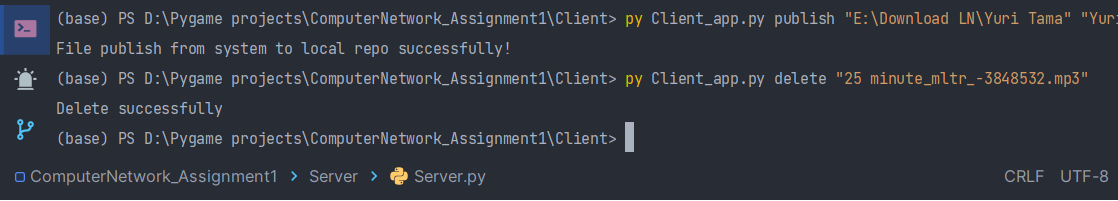
\includegraphics[width=0.7\textwidth]{tests/delete_command.png}
			\hspace{\textwidth}
			\caption{Câu lệnh \textbf{delete} từ client}
			\label{delete_command}
		\end{center}
	\end{figure}
	\newpage
	Kiểm tra lại trên server.
	\begin{figure}[h]
		\begin{center}
			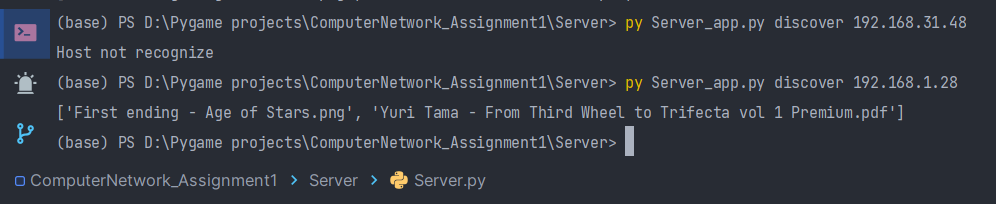
\includegraphics[width=0.8\textwidth]{tests/server_dis_af_delete.png}
			\hspace{\textwidth}
			\caption{Câu lệnh \textbf{publish} từ client}
			\label{server_dis2_command}
		\end{center}
	\end{figure}
	\subsubsection{Truyền file từ một client sang client khác}
	Tiếp tục từ trường hợp phần trước, lần này có thêm một client mới (client 2) cũng publish một file của mình lên server.
	\begin{figure}[h]
		\begin{center}
			\begin{subfigure}[b]{0.4\textwidth}
				\centering
				\includegraphics[width=\textwidth]{tests/client_2_bf_publish.jpg}
				\hspace{\textwidth}
				\caption{Client 2 trước khi publish}
			\end{subfigure}
			\begin{subfigure}[b]{0.4\textwidth}
				\centering
				\includegraphics[width=\textwidth]{tests/client_2_af_publish.jpg}
				\hspace{\textwidth}
				\caption{Client 2 sau khi publish}
			\end{subfigure}
			\\
			\begin{subfigure}[b]{0.8\textwidth}
				\centering
				\includegraphics[width=\textwidth]{tests/client_2_publish_command.jpg}
				\hspace{\textwidth}
				\caption{Câu lệnh \textbf{publish} của client 2}
			\end{subfigure}
			\caption{Client 2 thưc thi câu lệnh \textbf{publish}}
		\end{center}
	\end{figure}
	\newpage
	Client 1 list tìm ra các client đã kết nối và discover client 2 để tìm file cần fetch. Client 1 tiến hành fetch một file từ client 2.\\
	\begin{figure}[h]
		\begin{center}
			\begin{subfigure}[b]{0.8\textwidth}				
				\centering
				\includegraphics[width=\textwidth]{tests/client_2_file_for_fetch.jpg}
				\hspace{\textwidth}
				\caption{File dùng để fetch của client 2}
			\end{subfigure}
			\\
			\begin{subfigure}[b]{0.4\textwidth}
				\centering
				\includegraphics[width=\textwidth]{tests/client_1_list_dis.png}
				\hspace{\textwidth}
				\caption{Câu lệnh \textbf{list} và \textbf{discover} của client 1}
			\end{subfigure}
			\begin{subfigure}[b]{0.4\textwidth}
				\centering
				\includegraphics[width=\textwidth]{tests/client_1_fetch.png}
				\hspace{\textwidth}
				\caption{Câu lệnh \textbf{fetch} của client 1}
			\end{subfigure}
			\caption{Client 1 thực thi câu lệnh \textbf{list, discover, fetch}}
		\end{center}
	\end{figure}
	\newpage
	Tương tự, client 2 cũng list và discover client 1 để tìm file cần fetch. Có thể thấy sau khi fetch file, client 1 cũng đồng thời publish file đó lên cho server cùng biết. Sau đó, client 2 tiến hành fetch một file từ client 1.
	\begin{figure}[h]
		\begin{center}
			\begin{subfigure}[b]{0.45\textwidth}
				\centering
				\includegraphics[width=\textwidth]{tests/client_1_file_for_fetch.png}
				\hspace{\textwidth}
				\caption{File dùng để fetch của client 1}
			\end{subfigure}
			\begin{subfigure}[b]{0.45\textwidth}
				\centering
				\includegraphics[width=\textwidth]{tests/client_2_fetch.jpg}
				\hspace{\textwidth}
				\caption{Câu lệnh \textbf{fetch} của client 1}
			\end{subfigure}
			\caption{Client 2 thực thi câu lệnh \textbf{fetch}}
		\end{center}
	\end{figure}
	\newpage
	\subsubsection{Ping từ server tới một client}
	Ping từ server tới một \textit{hostname}. Có thể thấy, trong trường hợp \textit{hostname} đó chưa từng kết nối với server thì server sẽ không nhận ra được \textit{hostname} đó.
	\begin{figure}[h]
		\begin{center}
			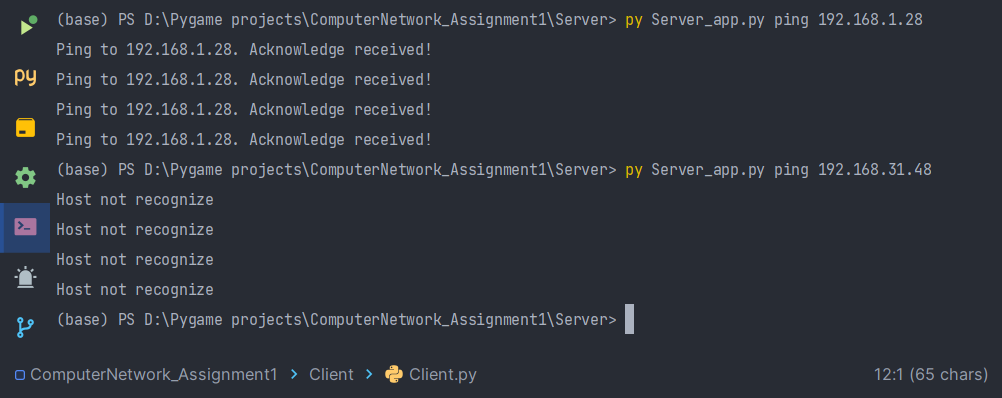
\includegraphics[width=0.7\textwidth]{tests/ping_command.png}
			\hspace{\textwidth}
			\caption{Câu lệnh \textbf{ping} từ server}
			\label{ping_command}
		\end{center}
	\end{figure}
	\subsubsection{Đánh giá theo mô tả trong bài tập lớn 1}
	\begin{enumerate}
		\item Chương trình đã xây dựng được một ứng dụng theo kiểu mạng P2P.
		\item Các chức năng chính được nêu trong phần mô tả bài tập lớn đã được hiện thực và hoạt động bình thường.
		\item Các client có thể gửi file tới nhiều client khác cùng một lúc.
		\item Xây dựng được một command line interpreter với câu lệnh tương ứng cho bên phía server lẫn client.
	\end{enumerate}
\end{document}

